\chapter{GPU Programming}

To achieve maximum performance, this project chooses to implement the fluid simulation software on GPUs. Originally built for graphics applications, GPUs were designed to handle a massive amount of geometries and pixels in parallel, because in graphics applications the computation for different geometries and pixels are largely independent. The ability to do massively parallel computation motivated GPGPU (General Purpose GPU) programming models to arise, which became significantly useful for scientific computing purposes. The implementation code in this project is written using the CUDA programming model, developed by the NVIDIA Corporation.

\section{The CUDA Programming Model}
CUDA employs the executing model known as SIMT (Single Instruction Multiple Thread). In this model, a large amount of GPU threads can be spawned simultaneously, each running the same sequence of code on different sets of data. GPU threads are organized in groups of 32, known as \textit{warps}, and the instructions running on threads of the same warp must be synchronized. However, different warps does not need to remain in sync. When the threads within a warp access the memory, the entire warp can be swapped out, so that a different warp can start executing before the memory access finishes. Using this mechanism, the GPU hides memory access latencies by allowing very fast context switching. As a result, each physical core in the GPU (known as a CUDA core) can simultaneously handle multiple logical threads.

As an example, the GPU used for development of this project is an NVIDIA GTX1060 Mobile, which contains 10 \textit{Streaming Multiprocessors}, each of which consists of 128 CUDA cores. Each streaming multiprocessors can have up to 2048 resident threads, giving a total of 20480 threads that can be simultaneously handled. Even though each GPU thread is not as fast as a CPU thread, a well adjusted CUDA program can still be up to 100 times faster than the same CPU program.


\begin{figure}[h]
    \centering
    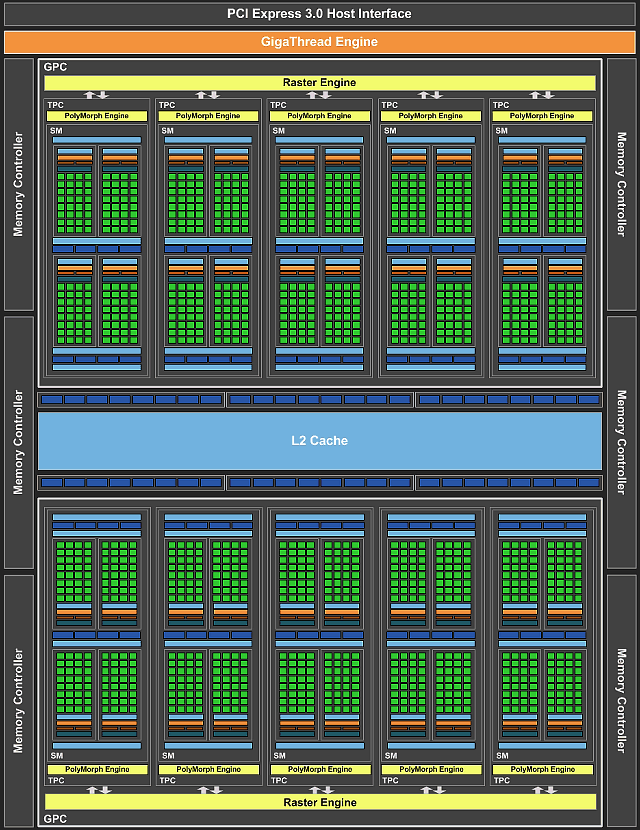
\includegraphics[width=11cm]{gp106}
    \caption{The architecture of a GTX 1060 (GP106), with 10 streaming multiprocessors, each containing 128 CUDA cores. Image courtesy to NVIDIA Corporation.}
    \label{figure GTX1060}
\end{figure}



\section{The OpenGL Render Pipeline}
\label{section opengl}

Since this project implements not only the simulation but also the rendering of fluids, the graphics functions of modern GPUs is also extensively utilized. Specifically, this program uses the OpenGL API for rendering.

In OpenGL (as well as other APIs such as Direct3D and Vulkan), the only types of geometries that can be rendered are points, lines, and triangles. For this reason, in order to render complex 3D objects, a mesh of triangles is often used to represent the surface of the object. After being fed into OpenGL's pipeline, these triangles go through 4 main stages:
\begin{enumerate}
    \item 
    \textit{The Vertex Shader}

    The vertex shader is a piece of GPU program, and its executed for each vertex of every triangle to be rendered. Usually, the vertex shader computes essential geometric information (e.g position on screen, normal) of the vertices, which are passed on to the next stage.
    
    \item 
    \textit{Rasterization}

    In the rasterization stage, a piece of hardware in the GPU uses the screen positions of vertices to determine, for each triangle, which pixels does the triangle cover. Each pixel of each triangle is then passed on to the next stage for colouring.
    
    \item
    \textit{The Pixel Shader}

    Also referred to as the \textit{fragment shader}, the pixel shader is also a piece of GPU program. The pixel shader culminates the job of the entire graphics pipeline: it computes of the colour of each pixel to be displayed.

    \item 
    \textit{Compositing}

    In 3D scene, objects might hide behind each other, and some pixels might be covered by multiple objects at different depth. The compositor's job is to determine which shading of the pixel to should be used, and in some cases (e.g opaque objects), how the differently shaded colours should be mixed together to give the final output. This process is essential to the multiphase fluid rendering algorithm invented in this project, to be described in subsection \ref{subsection multiphase render}.
    
\end{enumerate}

The full OpenGL pipeline includes a few extra stages, such as the geometry shader and the tesselation shader. However, these are optional stages and is not used in this project. In chapter \ref{chapter render}, more details will be given on the graphics pipeline of this project, and how it performs realistic liquid rendering in real time.